\section{Steady state solver} \label{sec:steady_state} 

In the absence of transients the discrete continuity equation \eqref{discrete_continuity_eqn} reduces to 
\begin{align}\label{discrete_steady_continuity_eqn}
\boxed{\mathbf{K}^T \mathbf{Q} = \mathbf{C}}
\end{align} 
and \eqref{discrete_momentum_eqn} reduces to 
\begin{align}\label{discrete_steady_momentum_eqn}
\boxed{\mathbf{R}(\mathbf{Q}, \mathbf{K} \mathbf{H}) = \mathbf{0} .}
\end{align}
We wish to solve \eqref{discrete_steady_continuity_eqn} along with the nonlinear momentum equations \eqref{discrete_steady_momentum_eqn}.

\subsection{Newton iteration}

Due to the nonlinear nature of \eqref{discrete_momentum_eqn} it is necessary to perform Newton iteration in order to converge to a solution. Let us split the flow rate and head vectors into a known/guessed part and a correction such that $\mathbf{Q} = \mathbf{Q}^g + \mathbf{Q}^c$ and $\mathbf{H} = \mathbf{H}^g + \mathbf{H}^c$ then 
\begin{align*}
\mathbf{R}(\mathbf{Q}, \mathbf{K} \mathbf{H}) \approx \mathbf{R}(\mathbf{Q}^g, \mathbf{K} \mathbf{H}^g ) + \pardiv{}{\mathbf{R}}{\mathbf{Q}} \Bigg\vert_{\mathbf{Q}^g} \mathbf{Q}^c + \pardiv{}{\mathbf{R}}{\mathbf{K} \mathbf{H}} \Bigg\vert_{\mathbf{K} \mathbf{H}^g} \mathbf{K} \mathbf{H}^c.
\end{align*}
The continuity equation \eqref{discrete_steady_continuity_eqn} is now given by
\begin{align}\label{discrete_steady_continuity_eqn_newton}
\mathbf{K}^T \mathbf{Q}^c = \mathbf{C} - \mathbf{K}^T \mathbf{Q}^g,
\end{align}
and the momentum equation \eqref{discrete_steady_momentum_eqn} is given by
\begin{align}\label{discrete_steady_momentum_eqn_newton}
- \pardiv{}{\mathbf{R}}{\mathbf{K} \mathbf{H}} \Bigg\vert_{\mathbf{K} \mathbf{H}^g} \mathbf{K} \mathbf{H}^c - \pardiv{}{\mathbf{R}}{\mathbf{Q}} \Bigg\vert_{\mathbf{Q}^g} \mathbf{Q}^c  = \mathbf{R}(\mathbf{Q}^g, \mathbf{K} \mathbf{H}^g).
\end{align}
These equations may be combined into a single system of the form
\begin{align}\label{discrete_steady_system}
\begin{bmatrix}
\mathbf{K}^T & \mathbf{0} \\
-\mathbf{J} & -\mathbf{G}
\end{bmatrix} 
\begin{bmatrix}
\mathbf{Q}^c \\ \mathbf{H}^c
\end{bmatrix} = \begin{bmatrix}
\mathbf{C} - \mathbf{K}^T \mathbf{Q}^g \\
\mathbf{R}(\mathbf{Q}^g, \mathbf{K} \mathbf{H}^g)
\end{bmatrix},
\end{align}
where $\mathbf{J} = \pardiv{}{\mathbf{R}}{\mathbf{Q}} \big\vert_{\mathbf{Q}^g}$ is the flow Jacobian matrix and $\mathbf{G} = \pardiv{}{\mathbf{R}}{\mathbf{K} \mathbf{H}} \big\vert_{\mathbf{K} \mathbf{H}^g} \mathbf{K}$. Boundary conditions specifying either the head or consumption at a node will modify this system of equations. 


\subsubsection{An example of the discrete calculus approach}

Consider the simple network shown in figure \ref{fig:discrete_calculus_example_network} which has $\mathbf{Q} = [Q_0, Q_1]^T$ and $\mathbf{H} = [H_0, H_1, H_2]^T$, along with
\begin{align*}
\mathbf{K} = \begin{bmatrix}
1 & -1 & 0 \\
0 & 1 & -1
\end{bmatrix}
\hspace{0.5cm} \text{and} \hspace{0.5cm} \mathbf{K}^T = \begin{bmatrix}
1 & 0  \\
-1 & 1 \\
0 & -1
\end{bmatrix}.
\end{align*}
We can see how the matrix product 
\begin{align*}
\mathbf{K}^T \mathbf{Q} = \begin{bmatrix}
1 & 0  \\
-1 & 1 \\
0 & -1
\end{bmatrix} \begin{bmatrix}
Q_0 \\ Q_1
\end{bmatrix} = \begin{bmatrix}
Q_0 \\ Q_1 - Q_0 \\ -Q_1
\end{bmatrix} = \mathbf{C}
\end{align*}
enforces that the sum of the flow rates into a node is equal to the consumption at that node. 

The system of equations (without boundary conditions) \eqref{discrete_steady_system} is given by
\begin{align*}
\begin{bmatrix}
1 & 0 & 0 & 0 & 0 \\
-1 & 1 & 0 & 0 & 0 \\
0 & -1 & 0 & 0 & 0 \\
-\pardiv{}{R}{Q}\big\vert_{Q_0^g} & 0 & -\pardiv{}{R}{\Delta H}\big\vert_{H_0^g - H_1^g} & \pardiv{}{R}{\Delta H}\big\vert_{H_0^g - H_1^g} & 0 \\
0 & -\pardiv{}{R}{Q}\big\vert_{Q_1^g} & 0 & -\pardiv{}{R}{\Delta H}\big\vert_{H_1^g - H_2^g} & \pardiv{}{R}{\Delta H}\big\vert_{H_1^g - H_2^g}
\end{bmatrix} \begin{bmatrix}
Q_0^c \\ Q_1^c \\ H_0^c \\ H_1^c \\ H_2^c
\end{bmatrix} = \begin{bmatrix}
C_0 - Q_0^g \\ 
C_1 - Q_1^g + Q_0^g \\ 
C_2 + Q_1^g \\ 
R\left(Q_0^g, H_0^g - H_1^g \right) \\ 
R\left(Q_1^g, H_1^g - H_2^g \right)
\end{bmatrix}.
\end{align*}
If we wished to specify head boundary conditions ($H_0 = H_{known} = 20$) at the first node and ($H_2 = P_{atm} / \rho g = 101325 / (999.7 \cdot 9.80665) = 10.33537514$) we would modify the system of equations to be 
\begin{align*}
\begin{bmatrix}
0 & 0 & 1 & 0 & 0 \\
-1 & 1 & 0 & 0 & 0 \\
0 & 0 & 0 & 0 & 1 \\
-\pardiv{}{R}{Q}\big\vert_{Q_0^g} & 0 & -\pardiv{}{R}{\Delta H}\big\vert_{H_0^g - H_1^g} & \pardiv{}{R}{\Delta H}\big\vert_{H_0^g - H_1^g} & 0 \\
0 & -\pardiv{}{R}{Q}\big\vert_{Q_1^g} & 0 & -\pardiv{}{R}{\Delta H}\big\vert_{H_1^g - H_2^g} & \pardiv{}{R}{\Delta H}\big\vert_{H_1^g - H_2^g}
\end{bmatrix} \begin{bmatrix}
Q_0^c \\ Q_1^c \\ H_0^c \\ H_1^c \\ H_2^c
\end{bmatrix} = \begin{bmatrix}
H_{known} - H_0^g \\ 
C_1 - Q_1^g + Q_0^g \\ 
\left( P_{atm} / \rho g \right) - H_2^g \\ 
R\left(Q_0^g, H_0^g - H_1^g \right) \\ 
R\left(Q_1^g, H_1^g - H_2^g \right)
\end{bmatrix}.
\end{align*}
The system of equations is then solved for the corrections, $\mathbf{Q}^c$ and $\mathbf{H}^c$, these are then used to update the guess $\mathbf{Q}^g \rightarrow \mathbf{Q}^g + \mathbf{Q}^c $ and $\mathbf{H}^g \rightarrow \mathbf{H}^g + \mathbf{H}^c $ and then process is repeated until the corrections are sufficiently small. Calculating the above example with two resistances being perfectly smooth pipes of lengths $L_0 = 100$m, $L_1 = 200$m and diameters $D_0=D_1=50$mm, with $C_1=0$, we obtain the solution $\mathbf{Q} = [0.00239623, 0.00239623]^T$ and $\mathbf{H} = [20, 16.77845838, 10.33537514]^T$. For such a simple example the system of equations is equivalent to the finite-difference form however for more complex networks, with multiple branches, the discrete calculus formulation allows the continuity condition to be satisfied without adding an additional constraint. 

\subsection{Resistances}

Each particular component in the network will have a different resistance term and different models of the same component may also produce different resistances. The typical resistance term for pipes is based on the Darcy-Weisbach equation and is shown in \eqref{pipe_resistance}. We will now outline some other resistance terms for common components. 

\subsubsection{Valves}

A valve has a discharge relationship defined by 
\begin{align}
Q = C_d A_v \sqrt{2 g \Delta H},
\end{align}
where $C_d$ is the discharge coefficient and $A_v$ is the valve opening area. Therefore 
\begin{align}
\Delta H = \frac{Q^2}{2g\left(C_d A_v \right)^2} = \frac{k Q^2}{2 g A^2} \implies \frac{k Q^2}{2A} - g A \Delta H = 0,
\end{align}
where $A$ is the cross-sectional area and $k$ is the loss coefficient which varies depending upon the percentage opening of the valve. This means that the resistance term for valves may be written as
\begin{align}
R_j = - \frac{k_j Q_j|Q_j| }{2 A_j} + g A_j \Delta H_j.
\end{align}
Alternatively we could write this resistance as 
\begin{align} \label{valve_resistance}
    \boxed{ R_j = - \frac{Q_j|Q_j| }{2 A_j} + k_j^{-1} g A_j \Delta H_j, }
\end{align}
but we must remember that in this form the transient coefficient in the matrix $\mathbf{B}$ is given by
\begin{align}
    \boxed{ B_{j,j} = k_j^{-1}. }
\end{align}
The loss coefficient $k$ may be determined from the discharge coefficient and the valve opening area using the relation 
\begin{align}
k = \frac{A^2}{\left(C_d A_v \right)^2} \implies k^{-1} = \frac{\left(C_d A_v \right)^2}{A^2} = k^{-1}(\tau),
\end{align}
where $\tau$ is the valve opening ratio. Writing the resistance function in the form \eqref{valve_resistance}, using $k^{-1}$, is more numerically stable as when the valve is fully closed, $A_v = 0$, $k \to \infty$ but $k^{-1} = 0$.

For example suppose we have a single valve resistance element with $H_0 = 20$, $H_1 = P_{atm} / \rho g$ with $k = 7$ and diameter $D = 50$mm. Then 
\begin{align}
Q =& \sqrt{\frac{2gA^2 \Delta H}{k}} = \pi D^2 \sqrt{\frac{g \left(H_0 - H_1 \right)}{8k}} \nonumber \\ =& \pi \cdot 0.05^2 \cdot \sqrt{\frac{9.80665 \cdot \left(20 - \left( \frac{101325}{ 997.0 * 9.80665} \right) \right)}{56}} \approx 0.010203.
\end{align} 
This solution agrees with the solution found from iteratively solving the linear system of equations. 

{\color{red} TODO inverse pressure loss coefficient $k^{-1}$ vs valve open percentage $\phi$ in a table.}


\subsubsection{Pumps}

In order to define the resistance term for a given pump we must know the relationship between the flow rate $Q$ and the pumping head $\Delta H$. It is necessary to know this relationship for both positive and negative heads and forward and reverse flow, i.e. in all four quadrants of the $(Q,\Delta H)$ diagram. Typically data for a given pump is only available in the first quadrant where $Q>0$ and $\Delta H > 0$ so it often necessary to extrapolate the data or use four-quadrant data from a similar pump. 

The discharge of a pump $Q$ is a function of the rotational speed $N$ and the pumping head $\Delta H$. The rotational speed of a pump during power failure is dependent upon the net torque $T$ and the combined moment of inertia of the rotating parts of the pump and the liquid entrained in the impeller. The values of these four variables at the best efficiency point are known as the rated conditions, denoted by a subscript $R$. Using the rated conditions as a reference we may define the non-dimensional variables
\begin{align*}
q = \frac{Q}{Q_R}, \hspace{0.5cm} \Delta h = \frac{\Delta H}{\Delta H_R}, \hspace{0.5cm} n = \frac{N}{N_R} \hspace{0.5cm} \text{and} \hspace{0.5cm} \tau = \frac{T}{T_R}.
\end{align*}

During normal pumping $q, \Delta H, n$ and $\tau$ are all positive, when one or more of these variables becomes negative the pump is in an abnormal operating zone. {\color{red} TODO Table of different zones + diagram - use Chaudry p119-120}. 

For pumps with similar geometry and flow profiles 
\begin{align*}
\frac{\Delta H}{N^2 D^2} = \text{Constant} \hspace{0.5cm} \text{and} \hspace{0.5cm} \frac{N}{Q D^3} = \text{Constant},
\end{align*}  
where $D$ is the diameter of the pump impeller. The impeller diameter $D$ is constant for a particular pump and so may be included in the constants therefore we may define the non-dimensional constants. 
\begin{align*}
\frac{\Delta h}{n^2} = \text{Constant} \hspace{0.5cm} \text{and} \hspace{0.5cm} \frac{n}{q} = \text{Constant}.
\end{align*} 

Let 
\begin{align*}
F_h = \frac{\Delta h}{n^2 + q^2}, \hspace{0.5cm} F_{\tau} = \frac{\tau}{n^2 + q^2} \hspace{0.5cm} \text{and} \hspace{0.5cm} \theta = \arctan\left( \frac{n}{q} \right), 
\end{align*}
then we may define four-quadrant characteristic curves for the head and torque for a particular pump. These curves define the functions $F_h(\theta)$ and $F_{\tau}(\theta)$ and are usually approximated using tabulated values given at equal intervals of $\theta$ {\color{red} TODO appendix containing example data table or reference table in Chaudry p523-524}. 

{\color{red} TODO discuss specific speed and how it can be used to describe similar pumps.}


So since $\Delta h = \left(n^2 + q^2 \right) F_h(\theta)$ it follows that 
\begin{align}
\Delta H = - \Delta H_R \left(n^2 + q^2 \right) F_h(\theta) \implies g A \Delta H_R \left(n^2 + q^2 \right) F_h(\theta) + g A \Delta H = 0,
\end{align}
therefore the resistance term for a pump defined by a four-quadrant characteristic curve is given by 
\begin{align}\label{pump_resistance}
\boxed{ R_j = g A_j \left[ \left( \Delta H_R \right)_j \left(n_j^2 + q_j^2 \right) F_h(\theta_j) + \Delta H_j \right], }
\end{align}
where $n_j = N_j / N_R$, $q_j = Q_j / Q_R$ and 
\begin{align*}
\theta = \arctan\left(\frac{n_j}{q_j} \right) = \text{atan2}(n_j, q_j),
\end{align*}
where if $\theta < 0$ then $\theta \rightarrow \theta + 2 \pi$. 
\subsubsection{Bends} 

Flow in curved pipes may be significantly impeded due to the effects of surface friction, secondary flow and flow separation. The resistance in a pipe bend may be modelled in a similar way to a valve but with the loss coefficient modified to account for the bend geometry and flow conditions. For a bend in a pipe $j$ of diameter $d_j$, bend angle $0 < \alpha_j < \pi$ and bend radius $r_j$, as shown in figure \ref{fig:bend_diagram}, the resistance may be defined by as
\begin{align}\label{bend_resistance}
\boxed{
  \!\begin{gathered}
  R_j = - \frac{k_j Q_j|Q_j| }{2 A_j} + g A_j \Delta H_j \hspace{0.5cm} \text{where}\\
  k_j = f_j \alpha_j \frac{r_j}{d_j}	 + (0.1 + 2.4 f_j) \sin \left( \frac{\alpha_j}{2} \right) + \frac{6.6 f_j \left[ \sqrt{\sin \left( \frac{\alpha_j}{2} \right) } + \sin \left( \frac{\alpha_j}{2} \right)  \right] }{\left(\frac{r_j}{d_j} \right)^{\frac{4 \alpha_j}{\pi}}}.
  \end{gathered}
}
\end{align}
Here $f_j = f(Q_j)$ is the friction factor which may also be a function of the pipe roughness. This empirical equation, see \cite{rennels22}, is one of a number of possible methods for determining loss coefficients for pipe bends; different methods may be preferred in certain situations. For equation \eqref{bend_resistance} to be valid it is required that $r_j / d_j \geq 0.5$.


\begin{figure}
\centering
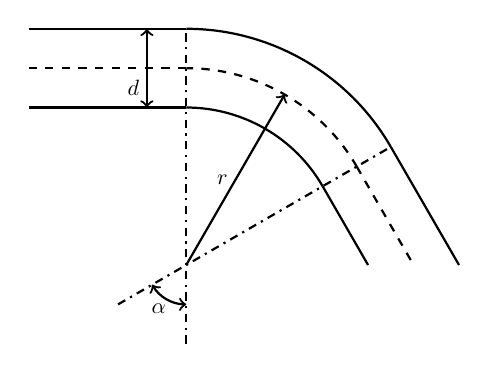
\begin{tikzpicture}[ scale=1, every node/.style={scale=0.8},] 
\draw[thick, dash dot] (0,-1) -- (0,3);
\draw[thick, dash dot] (-0.866,-0.5) -- (2.598,1.5);
% Inlet pipe
\draw[thick] (0,2) -- (-2,2);
\draw[thick, dashed] (0,2.5) -- (-2,2.5);
\draw[thick] (0,3) -- (-2,3);
% Bend
\draw[thick] (1.732,1) arc (30:90:2);
\draw[thick, dashed] (2.165,1.25) arc (30:90:2.5);
\draw[thick] (2.598,1.5) arc (30:90:3);
% Outlet pipe
\draw[thick] (1.732,1) -- (2.309,0);
\draw[thick, dashed] (2.165,1.25) -- (2.887,0);
\draw[thick] (2.598,1.5) -- (3.464,0);
% Annotations
\node[anchor=east] at (-0.5,2.25) {$d$};
\draw[thick, <->] (-0.5,2) -- (-0.5,3);
\draw[thick, <->] (-0.433,-0.25) arc (30:90:-0.5);
\node[anchor=north] at (-0.35,-0.39) {$\alpha$};
\draw[thick, ->] (0,0) -- (1.25,2.165);
\node[anchor=east] at (0.625,1.082) {$r$};
\end{tikzpicture} 
\caption{A bend in a pipe of diameter $d$ with a bend radius $r$ and bend angle $\alpha$.}
\label{fig:bend_diagram}
\end{figure}
\subsubsection{Size changes}

Flow through contractions/expansions cause the flow to accelerate/decelerate so it is important to consider size changes when pipes of different diameter are connected. Contractions and expansions are really two sides of the same coin, a contraction with flow in the opposite direction is an expansion just as an expansion with reverse flow is a contraction. Lets consider contractions and expansions separately before their action with reverse flow and combining them into a single component.  

\paragraph{Contraction}

Let us consider a contraction where the flow is from inlet node $i$ to outlet node $k$, as shown in figure \ref{fig:contraction_diagram}. The head loss due to the contraction \cite{rennels22} is given by
\begin{align}
H_L = \frac{K_c V_i^2}{2g},
\end{align}
where the contraction loss coefficient is
\begin{align*}
K_c = 0.0696 \left( 1 - \beta^2 \right) \lambda^2 + \left( \lambda - 1 \right)^2
\end{align*}
and
\begin{align*}
\lambda = 1 + 0.622 \left( 1 - 0.215 \beta^2 - 0.785 \beta^5 \right).
\end{align*}
Here $\beta = d_k / d_i$ is the ratio of the smaller diameter to the larger diameter and $V_i = Q_j / A_i$ is the inlet flow velocity. 

\begin{figure}
\centering
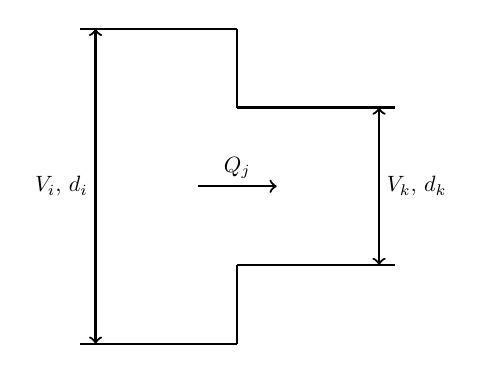
\begin{tikzpicture}[ scale=1, every node/.style={scale=0.8},] 
% Inlet pipe
\draw[thick] (0,0) -- (-2,0);
\draw[thick] (0,4) -- (-2,4);
% Contraction
\draw[thick] (0,0) -- (0,1);
\draw[thick] (0,4) -- (0,3);
% Outlet pipe
\draw[thick] (0,1) -- (2,1);
\draw[thick] (0,3) -- (2,3);
% Annotations
\node[anchor=east] at (-1.8,2) {$V_i$, $d_i$};
\draw[thick, <->] (-1.8,0) -- (-1.8,4);
\node[anchor=south] at (0,2) {$Q_j$};
\draw[thick, ->] (-0.5,2) -- (0.5,2);
\node[anchor=west] at (1.8,2) {$V_k$, $d_k$};
\draw[thick, <->] (1.8,1) -- (1.8,3);
\end{tikzpicture} 
\caption{An abrupt contraction where positive flow is from $i$ to $k$. The size ratio is $\beta = d_k / d_i$.}
\label{fig:contraction_diagram}
\end{figure}

\paragraph{Expansion}

For an expansion where the flow is from inlet node $i$ to outlet node $k$, as shown in figure \ref{fig:expansion_diagram} the head loss due to the expansion \cite{rennels22} is given by
\begin{align}
H_L = \frac{\hat{K}_e V_i^2}{2g},
\end{align}
where
\begin{align*}
\hat{K}_e = \left(1 - \hat{\beta}^2 \right)^2
\end{align*}
and $\hat{\beta} =  d_i / d_k$.

\begin{figure}
\centering
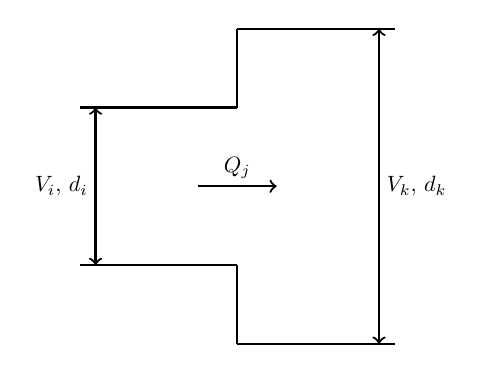
\begin{tikzpicture}[ scale=1, every node/.style={scale=0.8},] 
% Outlet pipe
\draw[thick] (0,0) -- (2,0);
\draw[thick] (0,4) -- (2,4);
% Contraction
\draw[thick] (0,0) -- (0,1);
\draw[thick] (0,4) -- (0,3);
% Inlet pipe
\draw[thick] (0,1) -- (-2,1);
\draw[thick] (0,3) -- (-2,3);
% Annotations
\node[anchor=west] at (1.8,2) {$V_k$, $d_k$};
\draw[thick, <->] (1.8,0) -- (1.8,4);
\node[anchor=south] at (0,2) {$Q_j$};
\draw[thick, ->] (-0.5,2) -- (0.5,2);
\node[anchor=east] at (-1.8,2) {$V_i$, $d_i$};
\draw[thick, <->] (-1.8,1) -- (-1.8,3);
\end{tikzpicture} 
\caption{An abrupt expansion where positive flow is from $i$ to $k$. The size ratio is $\hat{\beta} = d_i / d_k$.}
\label{fig:expansion_diagram}
\end{figure}

\paragraph{Reverse flow}

For positive flows, $Q_j > 0$, if $\beta < 1$ or $\hat{\beta} > 1$ then we have a contraction but if $\beta > 1$ or $\hat{\beta} < 1$ then we have an expansion. For negative flows, $Q_j < 0$, the situation is reversed if $\beta < 1$ or $\hat{\beta} > 1$ then we have an expansion but if $\beta > 1$ or $\hat{\beta} < 1$ then we have a contraction.

Reverse flow in a contraction, see figure \ref{fig:contraction_diagram}, is actually an expansion with a head loss given by
\begin{align}
H_L = \frac{K_e V_k^2}{2g},
\end{align}
where
\begin{align*}
K_e = \left(1 - \beta^2 \right)^2.
\end{align*}

Similarly reverse flow in an expansion, see figure \ref{fig:expansion_diagram}, is actually a contraction with a head loss given by
\begin{align}
H_L = \frac{\hat{K}_c V_k^2}{2g},
\end{align}
where 
\begin{align*}
\hat{K}_c = 0.0696 \left( 1 - \hat{\beta}^2 \right) \hat{\lambda}^2 + \left( \hat{\lambda} - 1 \right)^2
\end{align*}
and
\begin{align*}
\hat{\lambda} = 1 + 0.622 \left( 1 - 0.215 \hat{\beta}^2 - 0.785 \hat{\beta}^5 \right).
\end{align*}

\paragraph{Resistance for abrupt size changes}

These four different scenarios for forward/reverse flow and $\beta = \hat{\beta}^{-1}$ greater/less than $1$ means the resistance term for an abrupt size changes must be split into four parts. 
\begin{align}\label{abrupt_size_change_resistance}
\boxed{
  \!\begin{gathered}
  R_j = -\frac{K Q_j^2}{2 A} + g A \Delta H_j, \hspace{0.5cm} \text{where} \\
A = \begin{cases}
A_i &\text{if} \hspace{0.5cm} Q_j > 0,\\
A_k &\text{if} \hspace{0.5cm} Q_j < 0,
\end{cases} \nonumber \\
K = \begin{cases} 
K_c, &\text{if} \hspace{0.5cm} Q_j > 0, \beta < 1, \\
\hat{K}_e, &\text{if} \hspace{0.5cm} Q_j > 0, \beta > 1, \\
K_e, &\text{if} \hspace{0.5cm} Q_j < 0, \beta < 1, \\
\hat{K}_c, &\text{if} \hspace{0.5cm} Q_j < 0, \beta > 1.
\end{cases} \nonumber
  \end{gathered}
}
\end{align}
\subsubsection{Generic resistance}

Many components may be represented by a generic resistance of the form
\begin{align}
    \Delta H = A + B Q^n + C Q^m,
\end{align}
where $A$, $B$, $C$, $n$, and $m$ are constants. In order to preserve the directionality of the \ 
resistance, when the flow is reversed, we must replace $Q^n$ and $Q^m$ with $Q|Q|^{n-1}$ and \ 
$Q|Q|^{m-1}$, respectively. The resistance function for such a generic resistance may be written as
\begin{align} \label{generic_resistance}
    \boxed{ R_j = - g A_j \left[A + B Q_j|Q_j|^{n-1} + C Q_j|Q_j|^{m-1} \right] +  g A_j \Delta H_j. }
\end{align}
This form of resistance is fairly general and includes many common components when the coefficients \ 
and exponents are chosen appropriately. 



\subsubsection{Open pipes}

Open pipes are pipes that are open to the atmosphere at one end. The discharge relationship of an \ 
open pipe is given by 
\begin{align}
    \Delta H = \frac{K Q |Q|}{2 g A^2},
\end{align}
such that the resistance function is given by
\begin{align}
    R_j = - \frac{K Q_j |Q_j|}{2 A_j} + g A_j \Delta H.
\end{align}
Here the loss coefficient $K$ is a constant that depends on the geometry of the pipe at the exit. \
See \cite{rennels22} p.131 for details of different $K$ for various geometries.

% TODO do we need to have a different resistance for reverse flow?

%\cite{rennels22} (p131)
\subsubsection{Sprinklers}

\subsubsection{Flow controllers}

\subsubsection{Tee junctions}

\subsubsection{Cross junctions}

{\color{red} ETC -> other devices i.e. surge tanks, reservoirs, safety relief valve}

The solution of the steady state problem for flow networks has been thoroughly explored and many other solution methods exist. It is illustrative to see how the water-hammer equations collapse to the steady state problem in the absence of time variation but we must continue towards our original goal, to devise a method for calculating fluid transients in pipe networks. 

{\color{red} Appendix on calculating the laminar initial guess.}
